\documentclass{article}
\usepackage[utf8]{inputenc}

\title{Assignment 2}
\author{Benny Chen}
\date{\today}

\usepackage{color}
\usepackage{amsthm}
\usepackage{amssymb} 
\usepackage{amsmath}
\usepackage{listings}
\usepackage{xcolor}
\usepackage{listings}
\usepackage{graphicx}
\usepackage{enumitem}
\usepackage[hidelinks]{hyperref}

\definecolor{codegreen}{rgb}{0,0.6,0}
\definecolor{codegray}{rgb}{0.5,0.5,0.5}
\definecolor{codepurple}{rgb}{0.58,0,0.82}
\definecolor{backcolour}{rgb}{0.95,0.95,0.92}

\lstdefinestyle{mystyle}{
    backgroundcolor=\color{backcolour},   
    commentstyle=\color{codegreen},
    keywordstyle=\color{magenta},
    numberstyle=\tiny\color{codegray},
    stringstyle=\color{codepurple},
    basicstyle=\ttfamily\footnotesize,
    breakatwhitespace=false,         
    breaklines=true,                 
    captionpos=b,                    
    keepspaces=true,                 
    numbers=left,                    
    numbersep=5pt,                  
    showspaces=false,                
    showstringspaces=false,
    showtabs=false,                  
    tabsize=2
}

\lstset{style=mystyle}

\begin{document}

\maketitle

\section{Logistic Regression}

A country has two political parties, denoted by A and B here for simplicity. The probability that a voter votes for party A or party B is found to be modeled well by a 2-class logistic discrimination model with the following linear function:

\begin{equation}
    g(x) = 0.2x_1 + 0.1x_2 - 0.3x_3 -3
\end{equation}
\\
where $x_1$ is the family income (in \$10,000; if you are given \$20,000, $x_1 = 2$), $x_2$ is the number
of years of education, and $x_3$ is the gender (1 for male and 0 for female). Note that the sigmoid functionc an be written as $\frac{1}{1+\exp(-g(x))}$

The output y of the logistic discrimination model represents the probability that a column voter with attributes $x={(x_1; x_2; x_3)}^T$ will vote for party A.

\begin{enumerate}[label= (\alph*)]
    \item Consider a male voter with a family income of \$50,000 and 20 years of education. According to the model, what is the \emph{probability} that he will vote for party A\@?
    \item Consider a female voter with a family income of \$30,000 and 12 years of education. According to the model, what is the \emph{log odds (logit)} of the probability that she will vote for party A\@?
\end{enumerate}

\subsection*{Answer:}
\begin{enumerate} [label= (\alph*)]
    \item We first calculate the linear function $g(x)$:
    \begin{equation}
        g(x) = 0.2(5) + 0.1(20) - 0.3(1) - 3 = 0.3
    \end{equation}
    Then we plug $g(x)$ into the sigmoid function:
    \begin{equation}
        \frac{1}{1+\exp(-g(x))} = \frac{1}{1+\exp(-0.3)} = 0.574
    \end{equation}
    \item We first calculate the linear function $g(x)$:
    \begin{equation}
        g(x) = 0.2(3) + 0.1(12) - 0.3(0) - 3 = -1.2
    \end{equation}
    We then plug $g(x)$ into the sigmoid function:
    \begin{equation}
        \frac{1}{1+\exp(-g(x))} = \frac{1}{1+\exp(-(-1.2))} = 0.231
    \end{equation}
    We then calculate the log odds:
    \begin{equation}
        \ln(\frac{p}{1-p}) = \ln(\frac{0.231}{1-0.231}) = -1.2
    \end{equation}
    % \item The logit function is: 
    % \begin{equation}
    %     \ln(\frac{p}{1-p}) = x^{T}w+b
    % \end{equation}
    % We can plug in the values into the logit function:
    % \begin{equation}
    %     x = \begin{bmatrix}
    %         3 \\
    %         1 \\
    %         0
    %     \end{bmatrix}
    % \end{equation}
    % \begin{equation}
    %     w = \begin{bmatrix}
    %         0.2 \\
    %         0.1 \\
    %         -0.3
    %     \end{bmatrix}
    % \end{equation}
    % \begin{equation}
    %     b = -3
    % \end{equation}
    % \begin{equation}
    %     \ln(\frac{p}{1-p}) = \begin{bmatrix}
    %         3 \\
    %         1 \\
    %         0
    %     \end{bmatrix}^{T} \begin{bmatrix}
    %         0.2 \\
    %         0.1 \\
    %         -0.3
    %     \end{bmatrix} - 3 = 0.3
    % \end{equation}
\end{enumerate}

\section{Classification Evaluation Measures}

Consider a test data of 1000 samples with two classes: + class (100 samples) and $-$ class (900 samples). We have two random classifiers C1 and C2.
\\
We note that classifier C1 classifies test data to + class randomly with a probability p $(0 \le p \le 1)$ and classifier C2 classifies test data to + class randomly with a probability 2p.

\begin{enumerate}[label= (\alph*)]
    \item What is the expected TPR and FPR for C1 and C2\@?
    \item Is C2 a better classifier than C1? \emph{Hint: The random guess line in an ROC curve corresponds to TPR = FPR.}
\end{enumerate}

\subsection*{Answer:}
\begin{enumerate} [label= (\alph*)]
    \item Equations:
    $TRP = \frac{TP}{TP + FN}$, $FPR = \frac{FP}{FP + TN}$\\
    C1:
    $TP = \frac{100}{1000}p$
    $FN = \frac{100}{1000}(1-p)$
    $FP = \frac{900}{1000}p$
    $TN = \frac{900}{1000}(1-p)$
    \begin{equation}
        TPR = \frac{TP}{TP + FN} = \frac{p}{p + 1 - p} = \frac{p}{1} = p
    \end{equation}
    \begin{equation}
        FPR = \frac{FP}{FP + TN} = \frac{9p}{9p + 9 - 9p} = \frac{9p}{9} = p
    \end{equation}
    C2:
    $TP = \frac{100}{1000}2p$
    $FN = \frac{100}{1000}(1-2p)$
    $FP = \frac{900}{1000}2p$
    $TN = \frac{900}{1000}(1-2p)$
    \begin{equation}
        TPR = \\frac{TP}{TP + FN} = \frac{2p}{2p + 1 - 2p} = \frac{2p}{1} = 2p
    \end{equation}
    \begin{equation}
        FPR = \frac{FP}{FP + TN} = \frac{18p}{18p + 9 - 18p} = \frac{18p}{9} = 2p
    \end{equation}

    \item C2 is not a better classifier than C1 because the TPR and FPR are the same for both classifiers. 
\end{enumerate}

\section{Theory of Support Vector Machines}

\begin{enumerate}[label= (\alph*)]
    \item The following is the primal formualtion of L2 SVM (with squared slack variables), a variant of the standard SVM \@.
    \begin{equation}
        \min_{w,b,\xi} \frac{1}{2}w^{T}w + \frac{C}{2}\sum_{i=1}^{l}\xi_i^2
    \end{equation}
    \begin{equation}
        s.t. \quad y_i(w^{T}x_i + b) \ge 1 - \xi_i, \quad i \in \{1,\ldots,l\}, \quad \xi_i \ge 0, \quad i \in \{1,\ldots,l\}
    \end{equation}
    If we remove the last constraint ($\xi_i \ge 0$), we might get a simpler problem:
    \begin{equation}
        \min_{w,b,\xi} \frac{1}{2}w^{T}w + \frac{C}{2}\sum_{i=1}^{l}\xi_i^2
    \end{equation}
    \begin{equation}
        s.t. \quad y_i(w^{T}x_i + b) \ge 1 - \xi_i, \quad i \in \{1,\ldots,l\}
    \end{equation}
    Please provide the Lagrangian of the above simplified formulation.
    \item Please find the partial derivative of the Lagrangian in (a) with respect to $w$, $b$, and $\xi_i$.
\end{enumerate}

\subsection*{Answer:}
\begin{enumerate}
    \item The Lagrangian of the above simplified formulation is:
    \begin{equation}
        L(w,b,\xi,\alpha) = \frac{1}{2}w^{T}w + \frac{C}{2}\sum_{i=1}^{l}\xi_i^2 - \sum_{i=1}^{l}\alpha_i(y_i(w^{T}x_i + b) - 1 + \xi_i)
    \end{equation}

    \item The partial derivative of the Lagrangian in (a) with respect to $w$, $b$, and $\xi_i$ is:
    \begin{equation}
        \frac{\partial L}{\partial w} = w - \sum_{i=1}^{l}\alpha_i y_i x_i = 0
    \end{equation}
    \begin{equation}
        \frac{\partial L}{\partial b} = -\sum_{i=1}^{l}\alpha_i y_i = 0
    \end{equation}
    \begin{equation}
        \frac{\partial L}{\partial \xi_i} = \sum_{i=1}^{l}C \xi_i - \alpha_i = 0
    \end{equation}
\end{enumerate}

\section{Machine Learning Evaluation (ROC Curve)}

You have been asked to develop a classification model for diagnosing whether a patient is infected with a certain disease. To help you construct the models, your collaborator has provided you with a small training set (N = 10) with equal number of positive and negative examples. You tried several approaches and found two most promising models, C1 and C2. The outputs of the models in terms of predicting whether each of the training examples belong to the ``positive (+)'' class are summarized in the table below. The first row shows the probability a training example belongs to the positive class according to classifier C1, while the second row shows the same information for classifier C2. The last row indicates the true class label of the 10 training examples.
\\
\begin{table}[ht]
    \begin{tabular}{lllllllllll}
    $P(y=+|C_{1})$ & 0.1 & 0.15 & 0.2 & 0.3 & 0.31 & 0.4 & 0.62 & 0.77 & 0.81 & 0.95 \\
    $P(y=+|C_{2})$ & 0.25 & 0.49 & 0.05 & 0.35 & 0.66 & 0.6 & 0.7 & 0.65 & 0.55 & 0.99 \\
    y & $-$ & + & $-$ & $-$ & + & $-$ & + & + & $-$ & + 
    \end{tabular}
\end{table}
\\
For each model, we will evaluate different thresholds within the range of [0, 1], and a sample with probability $P(y = +|Cx)$ (x is either 1 or 2) that is lower than this threshold will be estimated as -, or + if greater than this threshold.
\\
By varying the thresholds (referred to the lecture slide on ROC), you can study the model performance and draw the ROC\@.

\begin{enumerate} [label= (\alph*)]
    \item Draw the corresponding ROC curves for both classifiers on the same plot.
    \item Which classifier can be considered better? Why?
\end{enumerate}

\subsection*{Answer:}
\begin{enumerate} [label= (\alph*)]
    \item 
    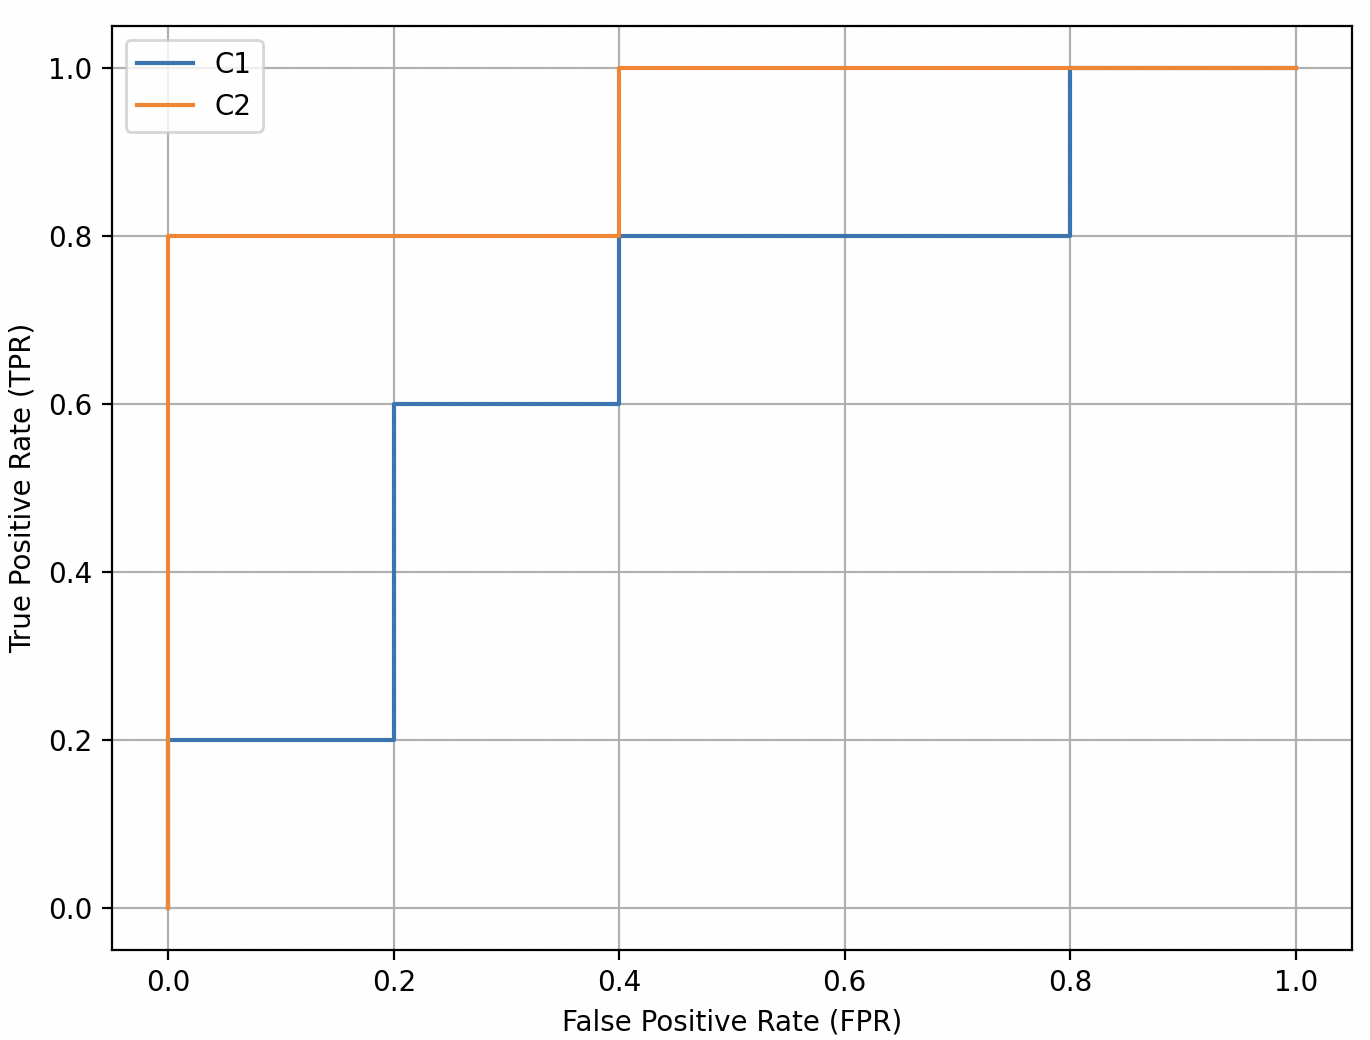
\includegraphics[scale=.4]{./images/ROC1.png}
    \item C2 is better because it has a higher AUC of 0.92 compared to C1's AUC of 0.68.
\end{enumerate}

\section{Clustering}

Consider the following set of one-dimensional data points:
$\{0.1,0.25,0.45,0.55,\\0.8,0.9\}$.
All the points are located in the range between $[0,1]$.

\begin{enumerate}[label= (\alph*)]
    \item Suppose we apply k-means clustering to obtain three clusters, A, B, and C. If the initial centroids are located at $\{0,0.4,1\}$, respectively, we have the following cluster assignment of the data points.
    \begin{table}[ht]
        \begin{tabular}{llllllllll}
        Iter & 0.10 & 0.25 & 0.45 & 0.55 & 0.80 & 0.90 & A & B & C \\
        0 & A & B & B & B & C & C & 0.00 & 0.40 & 1.00 \\
        1 & A & A & B & B & C & C & 0.1 & 0.42 & 0.85 \\ 
        2 & A & A & B & B & C & C & 0.18 & 0.5 & 0.85 \\ 
        3 & A & A & B & B & C & C & 0.18 & 0.5 & 0.85 
        \end{tabular}
    \end{table}

    Find the sum-of-squared error (SSE) of the clustering after the third iteration. And find the silhouette coefficient of data point 0.25 after the third iteration.

    \item For the dataset given in part (a), is it possible to obtain empty clusters? Why?
\end{enumerate}

\subsection*{Answer:}

\begin{enumerate}
    \item To calculate the SSE, we first calculate the distance between each point and its centroid:
    \begin{equation}
        d(0.1,0.18) = 0.0064
    \end{equation}
    \begin{equation}
        d(0.25,0.18) = 0.0049
    \end{equation}
    \begin{equation}
        d(0.45,0.5) = 0.0025
    \end{equation}
    \begin{equation}
        d(0.55,0.5) = 0.0025
    \end{equation}
    \begin{equation}
        d(0.8,0.85) = 0.0025
    \end{equation}
    \begin{equation}
        d(0.9,0.85) = 0.0025
    \end{equation}
    Then we sum them up to get the SSE\@:
    \begin{equation}
        SSE = 0.0064 + 0.0049 + 0.0025 + 0.0025 + 0.0025 + 0.0025 = 0.0213
    \end{equation}

    The formula for silhouette coefficient is:
    \begin{equation}
        s(i) = \frac{b(i) - a(i)}{\max\{a(i),b(i)\}}
    \end{equation}

    We first calculate $a(i)$:
    \begin{equation}
        a(i) = a(.25) = \frac{|.1 - .25|}{1} = 0.15
    \end{equation}
    We then calculate $b(i)$:
    \begin{equation}
        b(i) =  b(.25) = \min{\{\frac{.2 + .3}{2}, \frac{.55 + .65}{2}\}} = 0.25
    \end{equation}

    We can now calculate the silhouette coefficient:
    \begin{equation}
        s(i) = \frac{b(i) - a(i)}{\max\{a(i),b(i)\}} = \frac{0.25 - 0.15}{\max\{0.15,0.25\}} = 0.4
    \end{equation}

    \item No, it's not possible to have a empty cluster since the centroids will always have a point in the clusters.
\end{enumerate}
\end{document}